\documentclass{article}
\usepackage{graphicx} % Required for inserting images
\usepackage{hyperref}
\usepackage{tikz}
\usepackage{tabularray}
\usepackage{pgfplots}
\usepackage{float}

\title{Optimization of Numerical Functions Using the Hill Climbing Algorithm}
\author{Denis Crismariu}
\date{\today}

\begin{document}

\maketitle

\section{Abstract}
This report investigates the application of Hill Climbing and Simulated Annealing algorithms for optimizing mathematical functions. The study focuses on two variants of the Hill Climbing algorithm: First Improvement and Best Improvement. Through detailed experimentation, we evaluate the efficiency and accuracy of these methods. The results indicate that while the First Improvement variant is significantly faster, it tends to produce larger errors compared to the Best Improvement variant. Simulated Annealing, although slower than both Hill Climbing variants, sometimes provides better results but usually yields weaker outcomes. This report aims to provide insights into the trade-offs between speed and accuracy in local search algorithms and suggests potential areas for further research and improvement.

\section{Introduction}
This report details the use of the Hill Climbing and Simulated Annealing algorithms for optimizing mathematical functions. The study focuses on two variants of the Hill Climbing algorithm: First Improvement and Best Improvement. Through detailed experimentation, we evaluate the efficiency and accuracy of these methods. Specifically, our objective is to search for the minima of four benchmark functions: De Jong’s, Schwefel’s, Rastrigin’s, and Michalewicz’s.

The First Improvement variant of Hill Climbing quickly accepts the first neighboring solution that improves the objective function, making it 40\% faster but potentially 18\% less accurate. On the other hand, the Best Improvement variant evaluates all neighboring solutions and selects the best one, which generally leads to better solutions but at the cost of increased computational time. Simulated Annealing, although 200\% slower than Best Improvement variant, yields 10\% less error.

This report aims to provide a detailed analysis of these two Hill Climbing variants and Simulated Annealing, highlighting their strengths and weaknesses. By comparing their performance on the benchmark functions, we seek to understand the trade-offs involved and explore potential strategies for enhancing the algorithms' performance. The findings of this study could inform the development of more robust optimization techniques for a wide range of applications.

\section{Methods \& Implementation}

\subsection{Algorithm Used}
The Hill Climbing algorithm starts with an initial solution and makes incremental moves to find a better solution. If a move leads to a better solution, it is accepted; otherwise, it is rejected. Additionally, we employed the Simulated Annealing algorithm, which explores the solution space more broadly and can sometimes find better solutions.

\subsection{Implementation Choices}
The solutions are represented as vectors of real numbers, and neighbors are generated by flipping bits in the binary representation of the solutions. The initialization procedure involves generating random initial solutions, and the stopping condition is reached after a fixed number of epochs.

\subsection{Variants and Modifications}
We implemented two variants of the algorithm: Best Improvement and First Improvement. Best Improvement searches for the best neighbor in each iteration, while First Improvement accepts the first neighbor that improves the current solution. Additionally, we employed the Simulated Annealing algorithm, which explores the solution space more broadly and can sometimes find better solutions.

\subsection{Experimental Setup Description}
Experiments were conducted on well-known test functions: Rastrigin, Michalewicz, De Jong, and Schwefel. The dimensions used were 2, 5, and 10, and the precision was set to $10^{-5}$. Each experiment was repeated 10 times to ensure consistency of results.

\section{Experimental results}
The 4 benchmarked functions are the following:
\subsection{Rastrigin Function\cite{Rastrigin}}

$$ f(x) = A \cdot n + \sum_{i=1}^n \left[ x_i^2 - A \cdot cos(2 \pi x_i) \right],
A = 10, x_i \in \left[ -5.12, 5.15 \right]$$

The global minima is located at $f(x)=0; x(i)=0,  \forall i=1:n $
\begin{figure}[!h]
  \includegraphics[width=\textwidth,height=\textheight,keepaspectratio]{rastr.png}
  \caption{Rastrigin's Function\cite{rast_img}}
\end{figure}

\begin{table}[H]
\caption{Hill Climbing values based on 30 runs}
\begin{tblr}{
colspec={X[1,l] X[1,l] X[0.6,l] X[0.6,l]},
rowsep=0.01pt,  % Reduce the vertical padding between cell contents and borders
  cell{1}{1} = {c=2}{},
  cell{2}{1} = {r=4}{c},
  cell{6}{1} = {r=4}{c},
  cell{10}{1} = {r=4}{c},
  vlines,
  hline{1-2,6,10,14} = {-}{},
  hline{3-5,7-9,11-13} = {2-5}{},
}
     &              & HC Best & HC  First  & SA Best \\
D = 5 & Average error & 0.99496 & 0.99496 & 0.00007 \\
      &   Standard error & 0.50502 & 0.53057 & 0.49575 \\
      &   Min error & 0.00000 & 0.00000 & 0.00001 \\
      &   Max error & 1.00001 & 1.99497 & 0.99500 \\

D = 10 & Average error & 4.34619 & 5.45652 & 4.34377 \\
     &   Standard error & 0.85758 & 1.03037 & 1.13024 \\
     &   Min error & 2.23583 & 4.22070 & 1.99509 \\
     &   Max error & 5.98491 & 7.69236 & 6.22588 \\

D = 30 & Average error & 28.51616 & 36.63716 & 30.88161 \\
     &   Standard error & 2.50995 & 2.68096 & 2.50913 \\
     &   Min error & 20.78986 & 31.22622 & 24.59362 \\
     &   Max error & 31.90401 & 39.68781 & 34.73962 \\
\end{tblr}
\caption{Hill Climbing time (in seconds) based on 30 runs}
\begin{tblr}{
colspec={X[1,l] X[1,l] X[0.6,l] X[0.6,l]},
rowsep=0.01pt,  % Reduce the vertical padding between cell contents and borders
  cell{1}{1} = {c=2}{},
  cell{2}{1} = {r=4}{c},
  cell{6}{1} = {r=4}{c},
  cell{10}{1} = {r=4}{c},
  vlines,
  hline{1-2,6,10,14} = {-}{},
  hline{3-5,7-9,11-13} = {2-5}{},
}
     &              & HC Best & HC  First  & SA Best \\
D = 5 & Average time & 0.79450 & 0.49500 & 4.77250 \\
     &   Standard time & 0.01691 & 0.00200 & 0.01234 \\
     &   Min time & 0.76700 & 0.49100 & 4.75300 \\
     &   Max time & 0.83800 & 0.49900 & 4.80100 \\

D = 10 & Average time & 5.71550 & 3.20850 & 15.95050 \\
     &   Standard time & 0.06970 & 0.02373 & 0.05949 \\
     &   Min time & 5.65300 & 3.15500 & 15.86100 \\
     &   Max time & 5.92300 & 3.25900 & 16.10200 \\

D = 30 & Average time & 134.39850 & 74.28550 & 115.93400 \\
     &   Standard time & 2.23907 & 0.34071 & 2.34376 \\
     &   Min time & 129.82500 & 73.79400 & 115.36500 \\
     &   Max time & 136.28000 & 75.39900 & 125.26900 \\
\end{tblr}
\end{table}
\begin{figure}[H]%means place figure here, don't float it around, if possible
  \centering %inside a figure, centers the content
\begin{tikzpicture}
  \begin{axis}[
    height=0.25\textheight, % Set the height of the plot
    width=0.8\textwidth, % Set the width of the plot
      xlabel=dimensions,
      ylabel=time,
      legend pos=north west,
    ]
    \addplot [
      color=red, 
    ]
    coordinates {
     (5,0.79450)
     (10,5.71550)
     (30,134.39850)
    };
    \addlegendentry{Best Improvement}
    \addplot [
      color=blue,
    ]
    coordinates {
     (5,0.49500)
     (10,3.20850)
     (30,74.28550)
    };
    \addlegendentry{First Improvement}
    \addplot [
      color=orange,
    ]
    coordinates {
     (5,4.77250)
     (10,15.95050)
     (30,115.93400)
    };
    \addlegendentry{Simulated Annealing}

 \end{axis}
\end{tikzpicture}
\caption{Comparing average time of both methods}
\end{figure}

\subsection{Michalewicz Function\cite{michal}}

$$
f(x) = - \sum_{i=1}^n \sin \left(x_i \right)\sin^{2m}\left(\frac{ix_i^2}{\pi}\right),
x_i \in \left[ 0 , \pi \right]$$

The global minima is located at $n=5: f (x) = -4.687658$, for $n=10: f (x) = -9.66015$ and for  $n=30: f (x) = -29.6308839$\cite{glob_min}.

\begin{figure}[!h]
  \centering
  \includegraphics[width=\textwidth,height=\textheight,keepaspectratio]{michal.png}
  \caption{Michalewicz's Function\cite{michal_img}}
\end{figure}


\begin{table}[H]
\caption{Hill Climbing values based on 30 runs}
\begin{tblr}{
colspec={X[1,l] X[1,l] X[0.6,l] X[0.6,l]},
rowsep=0.01pt,  % Reduce the vertical padding between cell contents and borders
  cell{1}{1} = {c=2}{},
  cell{2}{1} = {r=4}{c},
  cell{6}{1} = {r=4}{c},
  cell{10}{1} = {r=4}{c},
  vlines,
  hline{1-2,6,10,14} = {-}{},
  hline{3-5,7-9,11-13} = {2-5}{},
}
     &              & HC Best & HC  First  & SA Best \\
D = 5 & Average error & 0.00070 & 0.00120 & 0.00071 \\
     &   Standard error & 0.00108 & 0.00435 & 0.00415 \\
     &   Min error & 0.00000 & 0.00000 & 0.00002 \\
     &   Max error & 0.00357 & 0.01839 & 0.02282 \\

D = 10 & Average error & 0.30218 & 0.36119 & 0.28258 \\
     &   Standard error & 0.08457 & 0.11373 & 0.10682 \\
     &   Min error & 0.10611 & 0.17242 & 0.01895 \\
     &   Max error & 0.45290 & 0.59881 & 0.45951 \\

D = 30 & Average error & 2.69373 & 3.22775 & 2.84582 \\
     &   Standard error & 0.22355 & 0.25850 & 0.29642 \\
     &   Min error & 2.03010 & 2.75044 & 1.88349 \\
     &   Max error & 3.03238 & 3.94261 & 3.43481 \\
\end{tblr}
\caption{Hill Climbing time (in seconds) based on 30 runs}
\begin{tblr}{
colspec={X[1,l] X[1,l] X[0.6,l] X[0.6,l]},
rowsep=0.01pt,  % Reduce the vertical padding between cell contents and borders
  cell{1}{1} = {c=2}{},
  cell{2}{1} = {r=4}{c},
  cell{6}{1} = {r=4}{c},
  cell{10}{1} = {r=4}{c},
  vlines,
  hline{1-2,6,10,14} = {-}{},
  hline{3-5,7-9,11-13} = {2-5}{},
}
     &              & HC Best & HC  First  & SA Best \\
D = 5 & Average time & 1.20600 & 0.83250 & 6.83750 \\
     &   Standard time & 0.03635 & 0.00638 & 0.01287 \\
     &   Min time & 1.14700 & 0.82000 & 6.80300 \\
     &   Max time & 1.26500 & 0.84200 & 6.88200 \\

D = 10 & Average time & 10.05350 & 5.70600 & 25.08550 \\
     &   Standard time & 0.25966 & 0.03323 & 0.03537 \\
     &   Min time & 9.12500 & 5.66600 & 25.03400 \\
     &   Max time & 10.44000 & 5.84900 & 25.20300 \\

D = 30 & Average time & 229.08950 & 123.95100 & 210.70550 \\
     &   Standard time & 4.39503 & 3.75969 & 0.89812 \\
     &   Min time & 225.80800 & 113.54100 & 208.88300 \\
     &   Max time & 239.06700 & 128.65300 & 211.16000 \\

\end{tblr}
\end{table}

\begin{figure}[H]%means place figure here, don't float it around, if possible
  \centering %inside a figure, centers the content
\begin{tikzpicture}
  \begin{axis}[
    height=0.25\textheight, % Set the height of the plot
    width=0.8\textwidth, % Set the width of the plot
      xlabel=dimensions,
      ylabel=time,
      legend pos=north west,
    ]
    \addplot [
      color=red, 
    ]
    coordinates {
     (5,1.20600)
     (10,10.05350)
     (30,229.08950)
    };
    \addlegendentry{Best Improvement}
    \addplot [
      color=blue,
    ]
    coordinates {
     (5,0.83250)
     (10,5.70600)
     (30,123.95100)
    };
    \addlegendentry{First Improvement}
    \addplot [
      color=orange,
    ]
    coordinates {
     (5,6.83750)
     (10,25.08550)
     (30,210.70550)
    };
    \addlegendentry{Simulated Annealing}

 \end{axis}
\end{tikzpicture}
\caption{Comparing average time of both methods}
\end{figure}

\subsection{De Jong Function\cite{dejong}}

$$
f(x) = \sum^n_{i=1}{x_i^2},
x_i \in \left[ -5.12 , 5.12 \right]
$$

The global minima is located at $f(x)=0; x(i)=0,  \forall i=1:n $

\begin{figure}[!h]
  \includegraphics[width=\textwidth,height=\textheight,keepaspectratio]{dejong.png}
  \caption{De Jong Function Function\cite{dejong_img}}
\end{figure}

\begin{table}[H]
\caption{Hill Climbing values based on 30 runs}
\begin{tblr}{
colspec={X[1,l] X[1,l] X[0.6,l] X[0.6,l]},
rowsep=0.01pt,  % Reduce the vertical padding between cell contents and borders
  cell{1}{1} = {c=2}{},
  cell{2}{1} = {r=4}{c},
  cell{6}{1} = {r=4}{c},
  cell{10}{1} = {r=4}{c},
  vlines,
  hline{1-2,6,10,14} = {-}{},
  hline{3-5,7-9,11-13} = {2-5}{},
}
     &              & HC Best & HC  First  & SA Best \\
D = 5 & Average error & 0.00000 & 0.00000 & 0.00001 \\
     &   Standard error & 0.00000 & 0.00000 & 0.00000 \\
     &   Min error & 0.00000 & 0.00000 & 0.00000 \\
     &   Max error & 0.00000 & 0.00000 & 0.00001 \\

D = 10 & Average error & 0.00000 & 0.00000 & 0.00004 \\
     &   Standard error & 0.00000 & 0.00000 & 0.00001 \\
     &   Min error & 0.00000 & 0.00000 & 0.00003 \\
     &   Max error & 0.00000 & 0.00000 & 0.00005 \\

D = 30 & Average error & 0.00000 & 0.00000 & 0.00062 \\
     &   Standard error & 0.00000 & 0.00000 & 0.00008 \\
     &   Min error & 0.00000 & 0.00000 & 0.00049 \\
     &   Max error & 0.00000 & 0.00000 & 0.00080 \\
       
\end{tblr}
\caption{Hill Climbing time (in seconds) based on 30 runs}
\begin{tblr}{
colspec={X[1,l] X[1,l] X[0.6,l] X[0.6,l]},
rowsep=0.01pt,  % Reduce the vertical padding between cell contents and borders
  cell{1}{1} = {c=2}{},
  cell{2}{1} = {r=4}{c},
  cell{6}{1} = {r=4}{c},
  cell{10}{1} = {r=4}{c},
  vlines,
  hline{1-2,6,10,14} = {-}{},
  hline{3-5,7-9,11-13} = {2-5}{},
}
     &              & HC Best & HC  First  & SA Best \\
D = 5 & Average time & 0.59550 & 0.36900 & 3.44900 \\
     &   Standard time & 0.01034 & 0.00212 & 0.01301 \\
     &   Min time & 0.58400 & 0.36300 & 3.43500 \\
     &   Max time & 0.61700 & 0.37100 & 3.47400 \\

D = 10 & Average time & 4.67100 & 2.40750 & 10.82400 \\
     &   Standard time & 0.21079 & 0.01719 & 0.07531 \\
     &   Min time & 4.21600 & 2.38700 & 10.64900 \\
     &   Max time & 4.91200 & 2.46700 & 10.92500 \\

D = 30 & Average time & 106.61050 & 53.71950 & 76.09900 \\
     &   Standard time & 1.25481 & 0.54479 & 0.81151 \\
     &   Min time & 102.92200 & 52.77300 & 75.73100 \\
     &   Max time & 107.81200 & 54.54600 & 79.25700 \\
\end{tblr}
\end{table}

\begin{figure}[H]%means place figure here, don't float it around, if possible
  \centering %inside a figure, centers the content
\begin{tikzpicture}
  \begin{axis}[
    height=0.25\textheight, % Set the height of the plot
    width=0.8\textwidth, % Set the width of the plot
      xlabel=dimensions,
      ylabel=time,
      legend pos=north west,
    ]
     \addplot [
      color=red, 
    ]
    coordinates {
     (5,0.59550)
     (10,4.67100)
     (30,106.61050)
    };
    \addlegendentry{Best Improvement}
    \addplot [
      color=blue,
    ]
    coordinates {
     (5,0.36900)
     (10,2.40750)
     (30,53.71950)
    };
    \addlegendentry{First Improvement}
    \addplot [
      color=orange,
    ]
    coordinates {
     (5,3.44900)
     (10,10.82400)
     (30,76.09900)
    };
    \addlegendentry{Simulated Annealing}

 \end{axis}
\end{tikzpicture}
\caption{Comparing average time of both methods}
\end{figure}


\subsection{Schwefel Function\cite{schwef}}

$$
f(x) = 418.9829n - \sum_{i=1}^n{x_i\sin(\sqrt{\left|x_i\right|})},
x_i \in \left[ -500 , 500 \right]
$$

The global minima is located at $f(x)=0; x(i)=0,  \forall i=1:n $

\begin{figure}[!h]
  \includegraphics[width=\textwidth,height=\textheight,keepaspectratio]{schwef.png}
  \caption{Schwefel's Function\cite{schwef_img}}
\end{figure}

\begin{table}[H]
\caption{Hill Climbing values based on 30 runs}
\begin{tblr}{
colspec={X[1,l] X[1,l] X[0.6,l] X[0.6,l]},
rowsep=0.01pt,  % Reduce the vertical padding between cell contents and borders
  cell{1}{1} = {c=2}{},
  cell{2}{1} = {r=4}{c},
  cell{6}{1} = {r=4}{c},
  cell{10}{1} = {r=4}{c},
  vlines,
  hline{1-2,6,10,14} = {-}{},
  hline{3-5,7-9,11-13} = {2-5}{},
}
     &              & HC Best & HC  First  & SA Best \\
D = 5 & Average error & 0.10484 & 34.23671 & 0.10448 \\
     &   Standard error & 0.09134 & 28.68144 & 0.09440 \\
     &   Min error & 0.00072 & 0.00131 & 0.00077 \\
     &   Max error & 0.31107 & 118.54224 & 0.31235 \\

D = 10 & Average error & 119.15130 & 305.85470 & 152.93740 \\
     &   Standard error & 55.84528 & 75.56549 & 51.43024 \\
     &   Min error & 0.52096 & 119.34473 & 34.54753 \\
     &   Max error & 187.32977 & 424.10354 & 234.58154 \\

D = 30 & Average error & 1221.76800 & 1812.85000 & 1243.47500 \\
     &   Standard error & 141.61020 & 154.69530 & 157.46650 \\
     &   Min error & 789.55774 & 1383.45220 & 805.87911 \\
     &   Max error & 1407.21618 & 2016.31897 & 1463.69494 \\
\end{tblr}
\caption{Hill Climbing time (in seconds) based on 30 runs}
\begin{tblr}{
colspec={X[1,l] X[1,l] X[0.6,l] X[0.6,l]},
rowsep=0.01pt,  % Reduce the vertical padding between cell contents and borders
  cell{1}{1} = {c=2}{},
  cell{2}{1} = {r=4}{c},
  cell{6}{1} = {r=4}{c},
  cell{10}{1} = {r=4}{c},
  vlines,
  hline{1-2,6,10,14} = {-}{},
  hline{3-5,7-9,11-13} = {2-5}{},
}
     &              & HC Best & HC  First  & SA Best \\
D = 5 & Average time & 1.73150 & 1.06200 & 6.77250 \\
     &   Standard time & 0.33685 & 0.00749 & 0.02612 \\
     &   Min time & 1.63000 & 1.05300 & 6.71300 \\
     &   Max time & 2.72500 & 1.09500 & 6.79700 \\

D = 10 & Average time & 14.02400 & 7.34200 & 22.64400 \\
     &   Standard time & 0.26543 & 0.11197 & 0.02968 \\
     &   Min time & 12.91900 & 6.83200 & 22.58300 \\
     &   Max time & 14.51100 & 7.37500 & 22.70400 \\

D = 30 & Average time & 334.32450 & 160.86850 & 171.21700 \\
     &   Standard time & 9.76273 & 0.91532 & 3.06020 \\
     &   Min time & 319.04200 & 160.15900 & 168.31700 \\
     &   Max time & 349.08300 & 164.24300 & 176.71400 \\
\end{tblr}
\end{table}

\begin{figure}[H]%means place figure here, don't float it around, if possible
  \centering %inside a figure, centers the content
\begin{tikzpicture}
  \begin{axis}[
    height=0.25\textheight, % Set the height of the plot
    width=0.8\textwidth, % Set the width of the plot
      xlabel=dimensions,
      ylabel=time,
      legend pos=north west,
    ]
        \addplot [
      color=red, 
    ]
    coordinates {
     (5,1.73150)
     (10,14.02400)
     (30,334.32450)
    };
    \addlegendentry{Best Improvement}
    \addplot [
      color=blue,
    ]
    coordinates {
     (5,1.06200)
     (10,7.34200)
     (30,160.86850)
    };
    \addlegendentry{First Improvement}
    \addplot [
      color=orange,
    ]
    coordinates {
     (5,6.77250)
     (10,22.64400)
     (30,171.21700)
    };
    \addlegendentry{Simulated Annealing}

 \end{axis}
\end{tikzpicture}
\caption{Comparing average time of both methods}
\end{figure}


\section{Comparing Methods}
Comparing First Improvement and Simulated Annealing methods to Best Improvement, we observed that First Improvement is usually faster but may not always find the optimal solution. Best Improvement, although slower, generally provides better solutions. Simulated annealing is slower than both but sometimes can even give better results; however, the results are usually weaker.

\section{Conclusions}
The Hill Climbing algorithm is effective for optimizing mathematical functions, but its performance depends on parameters and the variant used. Additionally, Simulated Annealing, while slower, can sometimes provide better results. In the future, it would be interesting to explore combinations with other optimization methods, such as Gradient Descent or Genetic Algorithms, to improve performance.







\begin{thebibliography}{9}

\bibitem{rast_img}
Authors: Sonja Surjanovic \& Derek Bingham, Simon Fraser University \\ Rastrigin's Function rendered image.
  \url{https://www.sfu.ca/~ssurjano/rastr.html}

\bibitem{Rastrigin}
  Rastrigin, L. A. "Systems of extremal control." Mir, Moscow (1974).

\bibitem{michal_img}
Authors: Sonja Surjanovic \& Derek Bingham, Simon Fraser University \\ Michalewicz's Function rendered image.
  \url{https://www.sfu.ca/~ssurjano/michal.html}

\bibitem{michal}
    Michalewicz, Zbigniew. "A survey of constraint handling techniques in evolutionary computation methods." (1995).

\bibitem{dejong_img}
Dejong's Function rendered image.
  \url{http://www.geatbx.com/docu/fcnindex-msh_f1_500-2.gif}

\bibitem{dejong}
De Jong, Kenneth Alan. An analysis of the behavior of a class of genetic adaptive systems. University of Michigan, 1975.

\bibitem{schwef_img}
Authors: Sonja Surjanovic \& Derek Bingham, Simon Fraser University \\ Schwefel's Function rendered image.
  \url{https://www.sfu.ca/~ssurjano/schwef.html}

\bibitem{schwef}
Bäck, Thomas, and Hans-Paul Schwefel. "An overview of evolutionary algorithms for parameter optimization." Evolutionary computation 1.1 (1993): 1-23.

\bibitem{glob_min}
Vanaret, Charlie, et al. "Certified global minima for a benchmark of difficult optimization problems." arXiv preprint arXiv:2003.09867 (2020).


\end{thebibliography} 

% \begin{tikzpicture}
%     \makeatletter
%     \pgfplotsset{
%         calculate offset/.code={
%             \pgfkeys{/pgf/fpu=true,/pgf/fpu/output format=fixed}
%             \pgfmathsetmacro\testmacro{(\pgfplotspointmeta *10^\pgfplots@data@scale@trafo@EXPONENT@y)*\pgfplots@y@veclength)}
%             \pgfkeys{/pgf/fpu=false}
%         },
%         every node near coord/.style={
%             /pgfplots/calculate offset,
%             yshift=-\testmacro
%         },
%     }
%     \pgfplotstableread{
%         0 1 1 2 2 3 3
%         1 1 1 7 7 7 7
%         2 1 1 5.6 5.6 7.8 7.8 
%     }\dataset

%     \begin{axis}[
%         ybar,
%         width=16cm,
%         height=10cm,
%         ymin=0,
%         ymax=20,        
%         ylabel={Comparing To HC Best},
%         xtick=data,
%         xticklabels = {5 Dimensions, 10 Dimensions, 30 Dimensions},
%         xticklabel style={yshift=-13ex},
%         major x tick style = {opacity=0},
%         minor x tick num = 1,
%         minor tick length=0ex,
%         every node near coord/.append style={
%             anchor=east,
%             rotate=90
%         },
%         legend style={at={(1,1)}, anchor=north east},
%         legend entries={Time, Error}
%     ]
    
%     % Adding the plots with single label in the middle for each pair
%     \addplot[draw=black,fill=red!100] table[x index=0,y index=1] \dataset; 
%     \addplot[draw=black,fill=blue!100, nodes near coords={HC-B}] table[x index=0,y index=2] \dataset; 
    
%     \addplot[draw=black,fill=red!100] table[x index=0,y index=3] \dataset; 
%     \addplot[draw=black,fill=blue!100, nodes near coords={HC-F}] table[x index=0,y index=4] \dataset;
    
%     \addplot[draw=black,fill=red!100] table[x index=0,y index=5] \dataset; 
%     \addplot[draw=black,fill=blue!100, nodes near coords={SA}] table[x index=0,y index=6] \dataset;

%     \end{axis}
% \end{tikzpicture}%


\end{document}




